% This section details the code implemented in order to efficiently and effectively visualize simulation results in real time.
This section details the design employed to efficiently and effectively visualize simulation results in real-time.
% This is not related to the \shell{renderppm} subcommand, which uses CPU code to render a single simulation state as an image.

\subsection{Components}
There are four major components of the visualization which work together to create the final output.
\begin{itemize}
    \item CPU 0 - The Main Thread, which handles the CUDA simulation.
    \item CPU 1 - The Worker Thread, which records and enqueues Vulkan commands.
    \item The GPU, which executes both the CUDA and Vulkan commands.
    \item The Swapchain, which provides render targets that are displayed in the application window.
\end{itemize}
The GPU itself has three phases of execution, performed sequentially for each frame (\cref{tab:gpuexecution}).
Each frame accesses a set of per-frame data, which is reused in a circular buffer.
Each phase for the frame will use this data.
\begin{table}[h]
    \centering
    \begin{tabular}{l|c}
    Name & Abbreviation \\
    \hline
    Simulation & Sim \\
    Visualization Compute (e.g. simulating particles) & VizComp \\
    Visualization Graphics & VizGfx \\
    \end{tabular}
    \caption{GPU Execution Phases, with abbreviations}
    \label{tab:gpuexecution}
\end{table}

A key design goal with the visualization was to maximize GPU utilization.
The CPU work is much less complicated than the GPU work, so the CPU should always be able to keep the GPU fed with new work.
If the CPU failed to do this, the GPU would waste time idling when it could be doing useful work.

\begin{figurepage}
\begin{figure}[p]
    \centering
    \makebox[\textwidth][c]{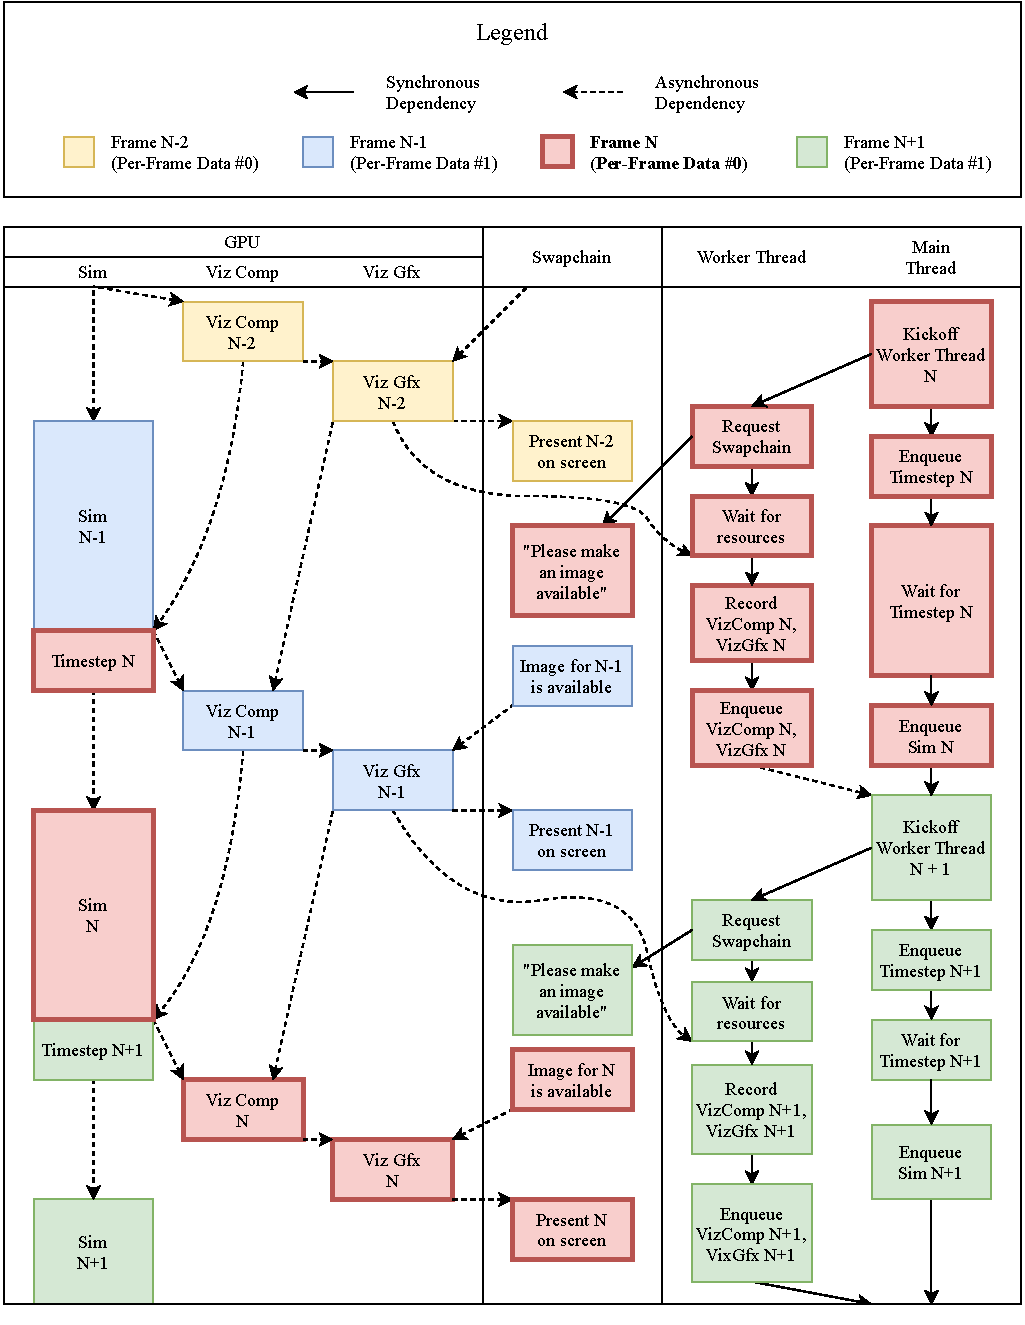
\includegraphics[width=1\linewidth]{Ch42Design/figures/FinalReport_Timing_Cropped.pdf}}
    \caption{Timing Breakdown of four visualization frames, assuming two sets of per-frame data}
    \label{fig:DesignTiming}
\end{figure}
\end{figurepage}

\subsection{Timing Breakdown}\label{sec:Design:Viz:Timing}

\cref{fig:DesignTiming} shows a breakdown of multiple frames of simulation and visualization, focusing on \textbf{frame \#N} which is highlighted in red.
It includes both synchronous and asynchronous dependencies.
A task with synchronous dependencies starts immediately once all dependencies finish.
A task with asynchronous dependencies can only start once all dependencies are finished, but may not start until later.

The main thread begins by initiating the worker thread before handling the simulation.
Before any CUDA work is enqueued, a semaphore is used to create a dependency on a previous compute job (`Viz Compute $N - 2$'). % Semaphore computeFinishedCanSim.
This compute cycle and the incoming CUDA work will access the same per-frame data\footnote{Viz Gfx jobs don't access the raw simulation buffers, so it doesn't delay the simulation.}, so this dependency prevents the simulation from writing to the data while the compute job reads from it.
For higher efficiency, this dependency could be inserted on `Sim $N$' instead, but it would not affect the results in practice.

The \code{VulkanTickedRunner} enqueues CUDA work to determine the maximum timestep for the next tick (`Timestep $N$' in the diagram), waits to get the results back on the CPU, and enqueues the rest of the simulation based on the calculated timestep (`Sim $N$')\footnote{`Sim' and `Timestep' work are enqueued on the same CUDA stream, so they are implicitly ordered.}.
%\todocite{CUDA stream ordered}
If visualization requested a larger timestep than the calculated maximum, the process would be repeated until the total requested timestep had elapsed.
Once `Sim $N$' is finished, it signals a semaphore to allow `Viz Comp $N$' to continue the frame. % Semaphore simFinishedCanCompute

% The worker thread asks the swapchain for an image using the \code{vkAcquireNextImageKHR} function.
The worker thread uses the \code{vkAcquireNextImageKHR} function to ask the swapchain\footnote{The swapchain is a set of images provided by the OS that are shown in the windowing system} for an image.
This returns the index of a swapchain image that will eventually become available, and a semaphore that will be signalled once this happens.
Before `Viz Gfx $N$' can render to this image, it has to wait for this semaphore to signal it is ready. % Semaphore imageAcquiredCanRender
The thread then waits for frame $N-2$ to finish using the Vulkan resources in Resource Set 0 before it uses them to record `Viz Comp $N$' and `Viz~Gfx~$N$'. % Fence frameCmdBuffersInUse
\clearpage

The Viz jobs use semaphores to guarantee ordering:
`Viz Gfx $N$' must start after `Viz Comp $N$' finishes, which must start after `Sim $N$' finishes. % Semaphore simFinishedCanCompute, computeFinishedCanRender
`Viz Comp $N$' also has to wait for `Viz Gfx $N - 1$' to finish to avoid race conditions - all `Viz Comp' and `Viz Gfx' jobs share global memory instead of per-frame memory to avoid data copying. % Semaphore renderFinishedNextFrameCanCompute
Once `Viz Gfx $N$' finishes, it signals a semaphore to tell the swapchain/OS to present the newly rendered frame to the screen.
The worker thread records and enqueues the above work for the GPU.
Once the worker thread has finished it signals the main thread, and once the main thread finishes enqueueing `Sim $N$' the process restarts.

It's worth noting that based on these dependencies some GPU work could theoretically run in parallel, such as `Viz Comp $N$' and `Timestep $N-1$'.
Unfortunately, in practice this doesn't happen.
Running parallel compute workloads is only supported on NVIDIA GPUs from the Ampere generation onwards\cite{nvidiaAmpereWhitepaper}, such as the RTX~3000 series, and is not supported on the researcher's GTX~1080.
% Running parallel compute workloads was introduced in the Ampere GPU generation \cite{nvidiaAmpereWhitepaper}, such as the RTX~3000 series, and is not supported on the researcher's GTX~1080.
This also affects the work breakdown, preventing smaller pieces of work (such as computations for separate visualization layers) from running in parallel.
In the future, this could be mitigated by using an Ampere-level GPU, or by running the simulation and visualization on separate GPUs.
%(converting the tightly-coupled visualization to a loosely-coupled one.)

\subsubsection{Synchronization}
Implementing the unlocked framerate (\cref{req:VizFlatOut}) without running the simulation faster than real-time required the time taken for each frame to be measured.
This is approximated by measuring the time between `Kickoff Worker Thread' tasks on the CPU.
Using this, the program predicts how long a simulation frame \emph{would} take, and combines that with the requested simulation rate\footnote{e.g. 120 simulation ticks per second} to predict if the next frame should be a simulation frame.

This restriction can be removed, to run with an unlocked simulation rate, in which case the average time per simulation frame is chosen as the timestep for the next simulation tick.
This is capped with sensible minimum/maximum limits to avoid instability from outliers.

% In order to implement an unlocked framerate without running the simulation faster than real-time, the time between frame `starts'\footnote{i.e. kicking off the worker thread} is measured to determine how long an average simulation frame takes. 
% The desired `simulations-per-second' is set by the user, and 

\subsection{Visualization Work Breakdown}\label{sec:Design:Viz:Breakdown}
As specified in the Requirements (\cref{sec:Requirements}) the selected visualization layers are the Background, Quantity-by-Scalar, Quantity-by-Vector, and Particle Simulation.
The Background and Quantity-by-Scalar layers are visualized at the same time for simplicity.
Accounting for this, the breakdown of required work for each layer is shown in \cref{fig:VizBreakdown}.

The Compute sections are implemented using Vulkan Compute Shaders\cite{TheKhronosGroupVulkanSpec}, which are nearly equivalent to CUDA Kernels and are invoked similarly.
The Graphics sections are implemented using Vertex and Fragment Shaders, where the Vertex Shader determines the onscreen positions of the vertices that make up a model, and the Fragment Shader determines the colour of the onscreen pixels between those vertices.

\begin{figure}[h]
    \centering
    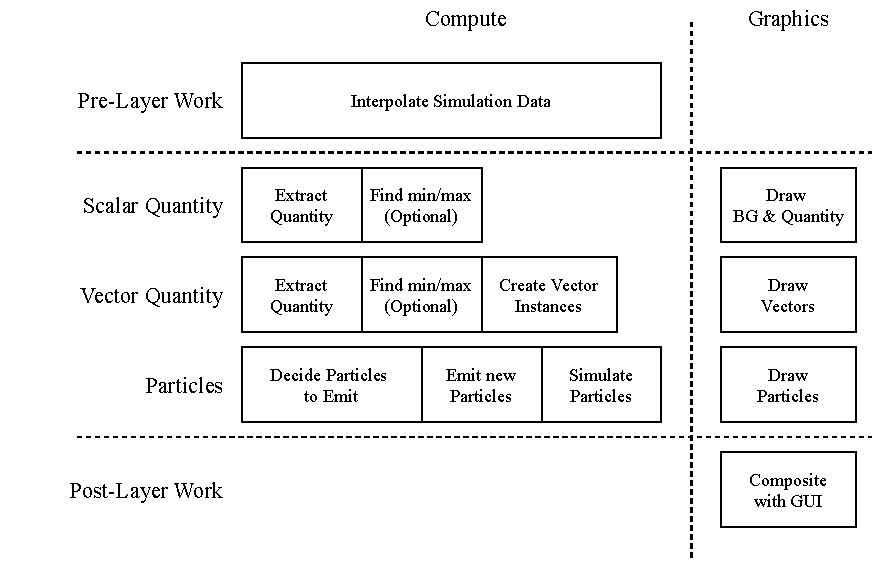
\includegraphics[width=\linewidth]{Ch42Design/figures/FinalReport_VizWork.pdf}
    \caption{Visualization Work Breakdown}
    \label{fig:VizBreakdown}
\end{figure}

\subsubsection{Data Interpolation}
The simulation stores data on a staggered grid (\cref{fig:staggered_grid}), but this is inconvenient for the visualization.
%not amenable for some visualization tasks.
The first step of the visualization is to move the exposed simulation data into a 2x resolution texture, applying interpolation where necessary, allowing the GPU to sample the exposed data at arbitrary points using the texture filtering hardware.
This applies trilinear interpolation, as required for the particle simulation.

\subsubsection{Auto-ranging}
Both Quantity-by-Scalar and Quantity-by-Vector have an optional auto-range mode, where the minimum and maximum values for the quantity are calculated and used instead of the user-defined range.
% Both Quantity-by-Scalar and Quantity-by-Vector have an optional auto-range mode, where the minimum and maximum values for the quantity are calculated instead of using the user-defined range.
This requires a GPU reduction, which is implemented in Vulkan just like it is in CUDA, using the second kernel of \cite{CUDAParallelReduction}.
To simplify the rendering code, in both cases the selected quantity is extracted to two buffers using a specialized compute shader.
The first buffer includes the quantity with a `fluidmask' which shows if the selected pixel is a fluid or obstacle, and is used for the rendering along with the reduction result.
The second buffer is used for the reduction, and contains a min/max property for each element.%, used as the input to the reduction.
% In order to easily render the data in both cases the selected quantity is extracted to two buffers using a specialized compute shader.

\subsubsection{Indirect Instanced Rendering}
% Quantity-by-Vector and the Particle Simulation use Instanced Rendering to 
For Quantity-by-Vector and the Particle Simulation, the final outputs are rendered using Instanced Rendering.
%\todocite{Instanced Rnedering}
% The same model is rendered $N$ times, and the Vertex Shader gets an `instance index' $0 \le i < N$.
% This index is used to look up the instance's position/orientation in a separate buffer.
The same model is rendered $N$ times, and the Vertex Shader uses an `instance index' $0 \le i < N$ to look up the instance's position/orientation.
%in a separate buffer.
This method is much faster than rendering each instance separately, as it requires fewer draw calls on the CPU.
\begin{figure}[t]
    \centering
    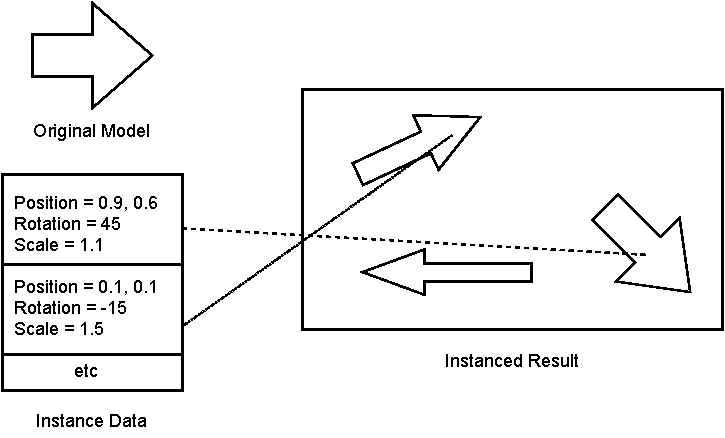
\includegraphics{Ch42Design/figures/FinalReport_InstancedRendering.pdf}
    \caption{Instanced Rendering Demonstration}
    \label{fig:InstancedRendering}
\end{figure}

When recording the command buffer on the CPU, the number of instances for both layers is not yet known.
For Quantity-by-Vector, the number of vectors is dependent on the simulation output.
%, because vectors cannot be placed on obstacles.
The previous visualization phase may kill some particles, so the particles cannot be predicted either.
% Some Particles may be killed in the previous visualization, so they 
% Some Particles may be killed by the previous round of simulation, so they cannot be predicted either.
To mitigate this, Indirect invocations are used for the vector/particle rendering and the particle simulation.
Instead of specifying the instance count at record time, a reference to a GPU buffer is used.
This GPU buffer contains the required parameters for the instanced rendering/compute dispatch, and can be atomically written by the GPU in a separate compute shader.

Creating new vectors/particle instances is done safely on the GPU using growable lists and atomic variables.
Each growable list consists of an array of values with a maximum length, and a `current size' variable.
When a value is added, the `current size' variable is incremented atomically, and the pre-increment value is then used to index the array and write the new instance parameter.
When a value is removed, the `current size' variable is decremented atomically, and the post-increment value can be used to see the deleted index.
Within a compute shader invocation, a list can only be growable or shrinkable but cannot be both.
Despite this limitation, the lists are suitable to implement the technique from \cite{WickedEngineParticles}.

\subsubsection{Final Composite}
As a final step, the visualization output is rendered with the other GUI elements.
This step is controlled by the Dear ImGUI library (see \cref{sec:LibrarySelection}).
An example of the visualization GUI is shown in \cref{fig:viz_gui}.

\begin{figure}[p]
    \centering
    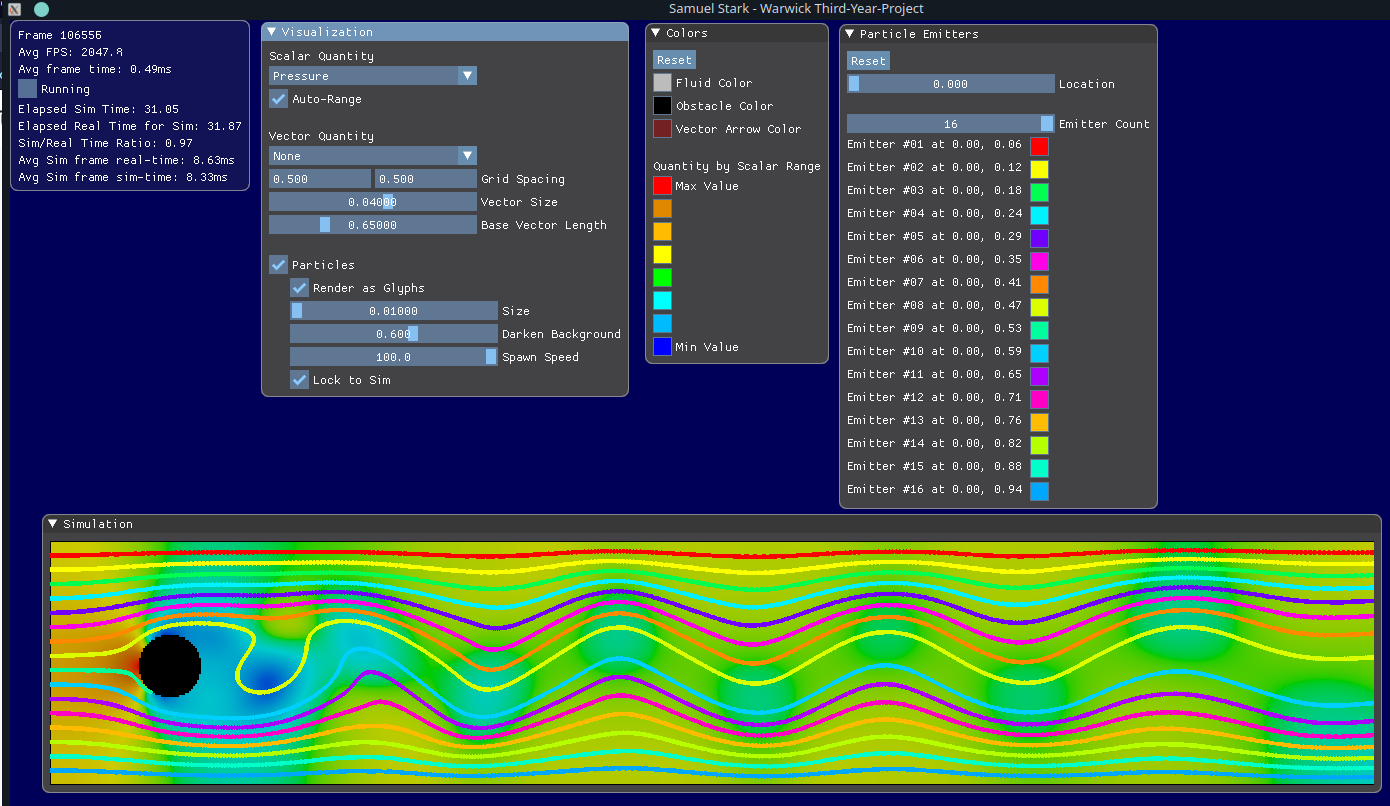
\includegraphics[width=\linewidth]{Ch42Design/figures/dan.png}
    \caption{Example of the Visualization GUI}
    \label{fig:viz_gui}
\end{figure}
\clearpage